\documentclass[12pt, a4paper]{article}
\usepackage[utf8]{inputenc}
\usepackage[english]{babel}
\usepackage{fancyhdr}
\usepackage{datetime}
\usepackage{hyperref}
\usepackage{longtable}
\usepackage{graphicx}
\usepackage{listings}
\usepackage{xcolor}
\usepackage{amsfonts}
\usepackage{amsmath}

\definecolor{mygreen}{rgb}{0,0.6,0}
\definecolor{mygray}{rgb}{0.5,0.5,0.5}
\definecolor{mymauve}{rgb}{0.58,0,0.82}
\lstset{ %
  language=[Sharp]C,
  backgroundcolor=\color{white},   % choose the background color
  basicstyle=\footnotesize,        % size of fonts used for the code
  breaklines=true,                 % automatic line breaking only at whitespace
  captionpos=b,                    % sets the caption-position to bottom
  commentstyle=\color{mygreen},    % comment style
  escapeinside={\%*}{*)},          % if you want to add LaTeX within your code
  keywordstyle=\color{blue},       % keyword style
  stringstyle=\color{mymauve},     % string literal style
}

\usepackage[font=small,labelfont=bf]{caption}
\hypersetup{
    colorlinks,
    citecolor=black,
    filecolor=black,
    linkcolor=black,
    urlcolor=black
}

\def\labelitemi{*}
\setcounter{tocdepth}{3}
\pagestyle{fancy}
\fancyhf{}
\renewcommand{\headrulewidth}{1pt}
\renewcommand{\footrulewidth}{1pt}
\rhead{\leftmark}
\rfoot{Page \thepage}

\graphicspath{{img}}

\begin{document}

\begin{titlepage}

    \newcommand{\HRule}{\rule{\linewidth}{0.5mm}} % Defines a new command for the horizontal lines, change thickness here
    
    \center % Center everything on the page
     
    %----------------------------------------------------------------------------------------
    %	HEADING SECTIONS
    %----------------------------------------------------------------------------------------
    
    \textsc{\LARGE Università Degli Studi Di Milano}\\[1.5cm] % Name of your university/college
    \textsc{\Large Artificial Intelligence For Video Games}\\[0.5cm] % Major heading such as course name
    %\textsc{\large Assignment 1}\\[0.5cm] % Minor heading such as course title
    
    %----------------------------------------------------------------------------------------
    %	TITLE SECTION
    %----------------------------------------------------------------------------------------
    
    \HRule \\[0.4cm]
    { \huge \bfseries Drunk Stride }\\[0.4cm] % Title of your document
    \HRule \\[1.5cm]
     
    %----------------------------------------------------------------------------------------
    %	AUTHOR SECTION
    %----------------------------------------------------------------------------------------
    
    \begin{minipage}{0.4\textwidth}
    \begin{flushleft} \large
    \emph{Author:}\\
    Giovanni \textsc{Cocco} \\
    \end{flushleft}
    \end{minipage}
    ~
    \begin{minipage}{0.4\textwidth}
    \begin{flushright} \large
    \emph{Academic year:} \\
    2023-2024\\
    \end{flushright}
    \end{minipage}\\[2cm]
    
    % If you don't want a supervisor, uncomment the two lines below and remove the section above
    %\Large \emph{Author:}\\
    %John \textsc{Smith}\\[3cm] % Your name
    
    %----------------------------------------------------------------------------------------
    %	DATE SECTION
    %----------------------------------------------------------------------------------------
    
    {\large \today}\\[4cm] % Date, change the \today to a set date if you want to be precise
    
    %----------------------------------------------------------------------------------------
    %	LOGO SECTION
    %----------------------------------------------------------------------------------------
    
   
\includegraphics[width=130px, keepaspectratio]{unimi}\\[1cm] % Include a department/university logo - this will require the graphicx package
     
    %----------------------------------------------------------------------------------------
    
    \vfill % Fill the rest of the page with whitespace
    
    \end{titlepage}

\clearpage
\tableofcontents{}
\listoffigures
\lstlistoflistings
\clearpage

\begin{abstract}
\noindent The project goal was to create an agent roaming on a platform while never moving along a straight line. More details were provided by the professors as follows:
\begin{itemize}
\item The platform can be of any size; square or rectangular.
\item The agent will change trajectory at random intervals. Each time the agent will travel over a
circumference leading first to right then to the left, then to the right again … and so on.
\item The agent is moving at a constant speed of 1 meter per second.
\item At each interval, the agent will pick a random value for the time to the next trajectory change
in the range (0, 10] seconds. Note that 0 is excluded.
\item Then, the agent selects a random circumference leading right or left with a radius between 0
(excluded) and the maximum radius that is not making the agent fall off the platform.
\item The selection of the radius is independent of the time of the next trajectory change.
\item The agent never stops moving.
\item The system must work independently on the platform shape or size.
\end{itemize}
\end{abstract}

\section{Scene setup}
The project main scene is \textbf{Assets/Scenes/Main.unity}.
\subsection{Agent}
As the agent movement is quite simple and does not require any complex physical simulation \textbf{kinematic movement} was chosen. This means that the agent does not have any rigid body component and its movement is not managed
in any way by the Unity physics engine.
It should be noted that it is not affected by gravity, but given the constraint that the agent should never fall off the platform it makes no difference in the resulting behavior.\\\\
The agent still has a \textbf{capsule collider} that is used to determine its own radius to avoid having half of the agent off the platform.
\subsection{Platform}
The platform is a simple plane with a \textbf{mesh collider}, as the default plane uses this. The agent code will hold a reference to the platform mesh collider.\\\\
The platform size is quite small to better test the interaction at the edges and to allow to see the whole platform in the camera. Although bigger platform size lead to bigger radius giving more believable results.

\section{Agent script}
\subsection{Public attributes}
The Agent class has few public attributes to allow some configuration from the Unity inspector.
\begin{lstlisting}[caption={Public attributes}]
    [Range(0.5f, 20.0f)]
    public float maxDecisionInterval = 10.0f;
    [Range(0.1f, 10.0f)]
    public float speed = 1.0f;
    [Range(10.0f, 360*4.0f)]
    public float maxRotationSpeed = 360.0f;
    public bool drawDebugGizmos = false;
    public MeshCollider platform;
\end{lstlisting}
The \textbf{maxDecisionInterval} and \textbf{speed} are set to a default value as required by the specifications.\\\\
The value of \textbf{maxRotationSpeed} controls the maximum rotation speed, this is used to avoid unrealistic fast spinning when a minuscule radius is randomly selected.\\\\
The flag \textbf{drawDebugGizmos} enables the rendering of the maximum radius that is not making the agent fall off the platform and the current selected circular trajectory.\\\\
A reference to the platform \textbf{MeshCollider} allows querying for its size and rotation along the Y axis.
It would be possible to use a \textbf{Collider} reference instead making it working also with a \textbf{BoxCollider}, this choice however would make the support of rotations on the Y axis troublesome.\\\\
From a \textbf{Collider} it is only possible to query the \textbf{world aligned bounds} making it impossible to query the actual height and width of the platform.
As the platform is a plane and, by defaults, Unity uses a \textbf{MeshCollider} for planes it was preferred to maintain the support for rotations rather than supporting \textbf{BoxCollider} too.

\subsection{Private attributes}
The Agent class has 3 private attributes.
\begin{lstlisting}[caption={Private attributes}]
    private float _direction = 1.0f;
    private Vector3 _circleCenter;
    private float _circleRadius;
\end{lstlisting}
The attributes \textbf{\_circleCenter} and \textbf{\_circleRadius} keep track of the current selected trajectory to follow while \textbf{\_direction} alternates the values 1.0f and -1.0f to keep track if the agent is moving right or left.

\subsection{Decision procedure}
To choose the next circular trajectory at random intervals a \textbf{coroutine} was used.\\\\
The coroutine \textbf{ChooseNextCircle()} is an infinite loop that waits for a random amount of time, between \textbf{float.Epsilon} and \textbf{maxDecisionInterval}, at every iteration.\\\\
The coroutine is in charge of updating the values of \textbf{\_circleCenter} and \textbf{\_circleRadius}. The radius is random between the maximum radius minus the agent size and \textbf{float.Epsilon}.\\\\
The circle center is simply calculated displacing the current agent position left or right by the radius.\\\\
At every iteration \textbf{\_direction} is inverted.

\begin{lstlisting}[caption={Decision procedure}]
    void Start() {
        StartCoroutine(ChooseNextCircle());
    }

    private IEnumerator ChooseNextCircle() {
        while (true) {
            // Subtract the Agent radius to avoid having half the agent off the platform
            _circleRadius = Random.Range(float.Epsilon, MaxRadius(_direction)-GetComponent<Collider>().bounds.extents.x*0.5f);
            _circleCenter = transform.position + _direction*transform.right * _circleRadius;

            yield return new WaitForSeconds(Random.Range(float.Epsilon, maxDecisionInterval));
            _direction *= -1;
        }
    }
\end{lstlisting}

\subsection{Motion}
The agent motion is implemented in the \textbf{FixedUpdate} method simply by rotating the agent around the circle center.\\\\
The angle of the rotation (per second) is calculated based on the agent speed and the circle perimeter, capped to the \textbf{maxRotationSpeed}.
\begin{lstlisting}[caption={FixedUpdate}]
   void FixedUpdate() {
        // Cap the maximun rotation speed to avoid ultra fast spinning on small circles
        float degreePerSecond = Mathf.Min(360.0f * speed/(2.0f*_circleRadius*Mathf.PI), maxRotationSpeed);
        Quaternion rotation = Quaternion.AngleAxis(_direction * degreePerSecond * Time.fixedDeltaTime, Vector3.up);

        transform.position = rotation*(transform.position - _circleCenter) + _circleCenter;
        transform.rotation *= rotation;
    }
\end{lstlisting}

\subsection{Calculating the maximum safe radius}
The calculation of the maximum safe radius is divided in 4 steps:
\begin{enumerate}
\item Rotate the coordinate system to have the platform axis aligned.
\item Calculate the platform extents.
\item Calculate the maximum safe radius for every edge of the platform.
\item Return the minimum of the 4 safe radius calculated.
\end{enumerate}
\begin{lstlisting}[caption={MaxRadius}]
    private float MaxRadius(float direction) {
        // Apply the inverse of the platform rotation to get back to an axis aligned coordinate system
        Quaternion invRotation = Quaternion.Inverse(platform.transform.rotation);
        Vector3 position = invRotation*transform.position;
        Vector3 right = invRotation*transform.right;

        // Get the extends of the platform from the mesh as the collider bounds are AA in world space
        Vector3 extents = Vector3.Scale(platform.sharedMesh.bounds.extents, platform.transform.lossyScale);
        Vector3 min = invRotation*platform.transform.position - extents;
        Vector3 max = invRotation*platform.transform.position + extents;

        // Get the max radius for each edge, then return the minimun one
        float x1 = (position.x-min.x)/(1.0f-right.x*direction);
        float x2 = (max.x-position.x)/(1.0f+right.x*direction);
        float z1 = (position.z-min.z)/(1.0f-right.z*direction);
        float z2 = (max.z-position.z)/(1.0f+right.z*direction);

        return Mathf.Min(Mathf.Min(x1, x2), Mathf.Min(z1, z2));
    }
\end{lstlisting}
To get the platform extends we can query the \textbf{sharedMesh} bounds of the \textbf{MeshCollider} and scale them based on the platform \textbf{lossyScale}.
Note that unless the platform is no longer a rectangle the \textbf{lossyScale} is exact.\\\\
All the code in the project query informations when needed avoiding caching them to better allow for real time changes, while this can be changed to improve performances, for the scope of this project, the ability to see changes in real time was preferred.
\clearpage
\noindent To get the maximum radius for a single axis aligned edge we should consider the following situation:
\begin{center}
    \centering
    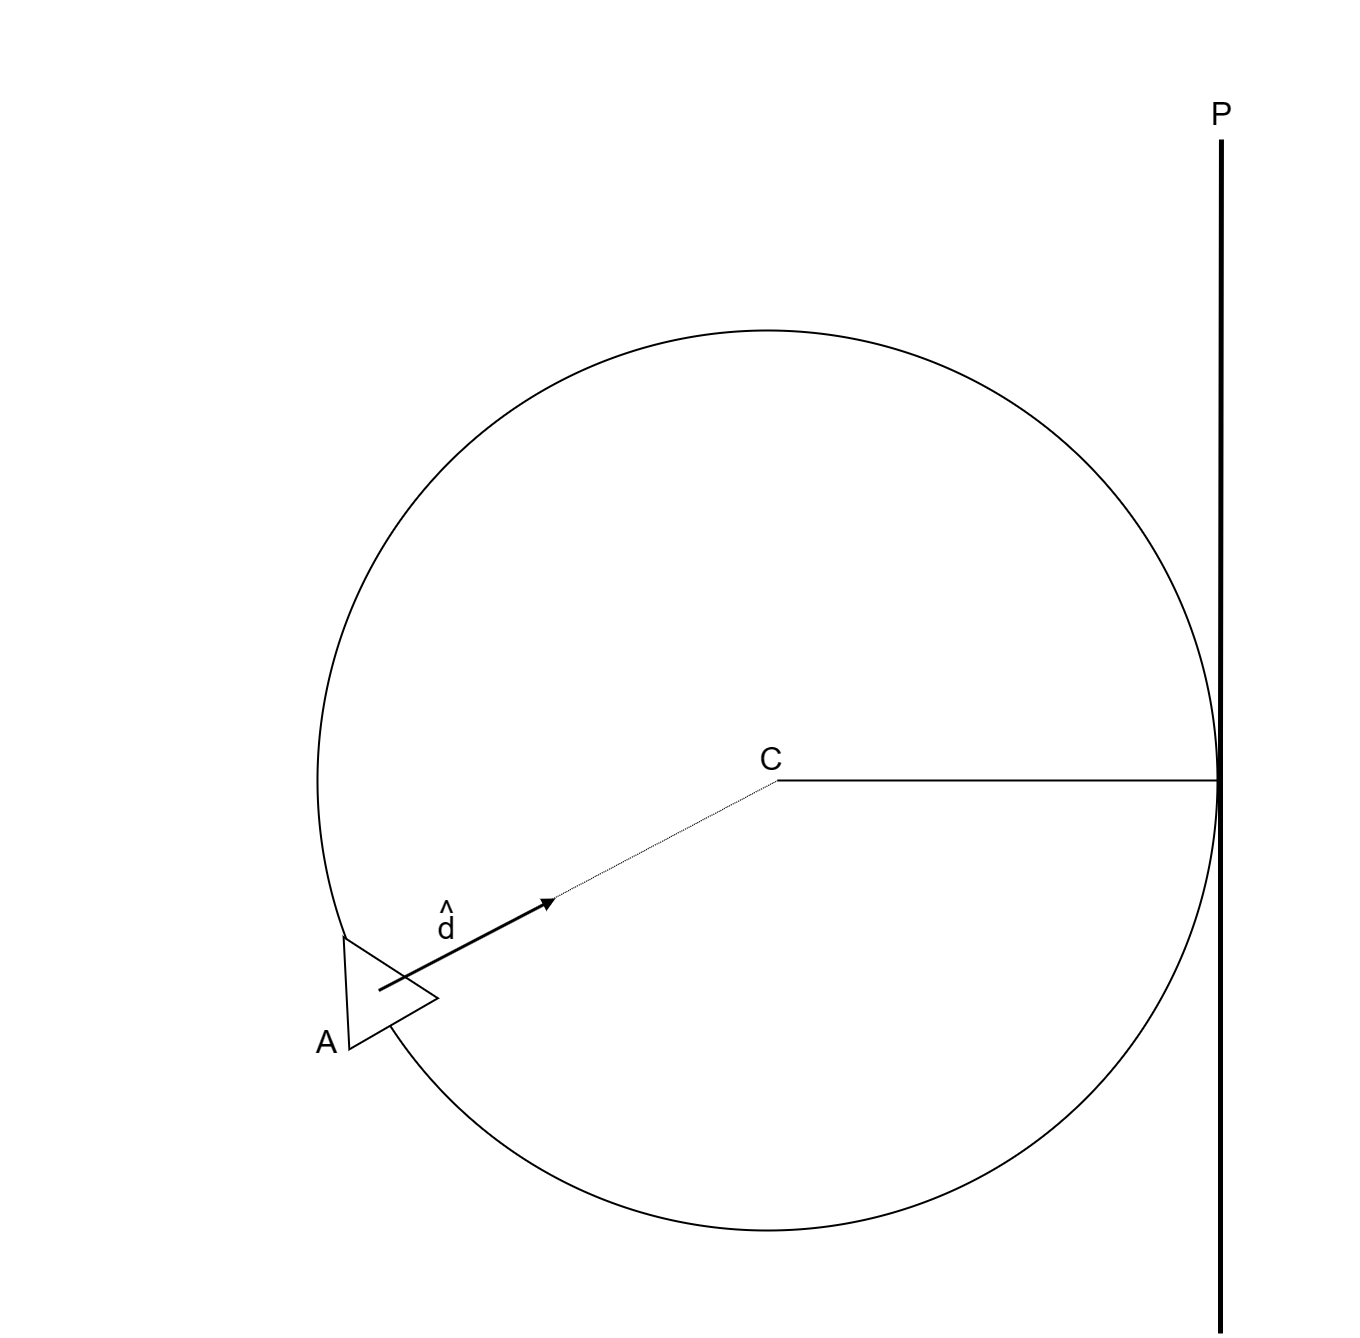
\includegraphics[width=0.75\textwidth]{draw.png}
    \captionof{figure}{Geometrical situation}
\end{center}
The center of the circle $C$ can be determinated from the agent position $A$, the radius $r$ and the right direction $\hat{d}$:
\[
C = A + r \hat{d}\text{, with }\|\hat{d}\|=1
\]
The radius $r$ is also the distance of the circle center from the platform border $P$, as we are axis aligned:
\[
r = P_x-C_x
\]
Putting all together:
\[
r = P_x - (A_x + r \hat{d}_x)
\]
Solving for $r$ we get:
\[
r = \dfrac{P_x-A_x}{1+\hat{d}_x}
\]
Note that in the project the agent center never reaches the edge of the platform, so the numerator can never be zero, and even if the denominator is zero we get, by floating point IEEE 754 arithmetic, an infinite value that will not get 
past the pick of the minimum of the 4 edges.\\\\
Mutatis mutandis for the other 3 edges.
\subsection{Gizmos}
To better debug the project Gizmos showing the maximum radius and the current trajectory were added with the following code:
\begin{lstlisting}[caption={Gizmos drawing}]
    void OnDrawGizmos() {
        if (drawDebugGizmos) {
            Vector3 offset = (platform.transform.position.y-transform.position.y+0.01f)*Vector3.up;
            Gizmos.color = Color.blue;
            DrawCircle(_circleCenter+offset, _circleRadius);
            Gizmos.color = Color.red;
            DrawCircle(transform.position+transform.right*MaxRadius(1.0f)+offset, MaxRadius(1.0f));
            DrawCircle(transform.position-transform.right*MaxRadius(-1.0f)+offset, MaxRadius(-1.0f));
        }
    }
\end{lstlisting}
The method \textbf{OnDrawGizmos()} get called even when the agent is not selected, this allows to see the maximum radius when editing the platform size, orientation and position from the editor.
\begin{center}
    \centering
    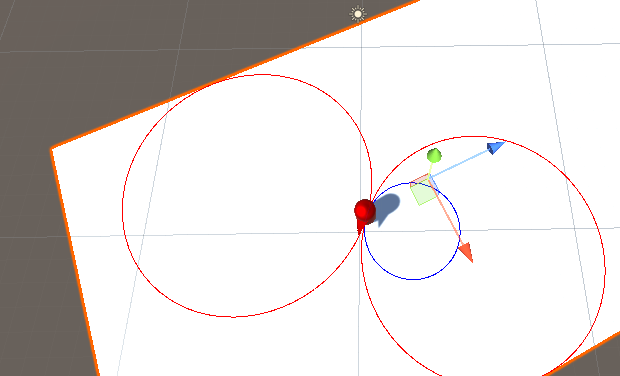
\includegraphics[width=0.8\textwidth]{gizmos.png}
    \captionof{figure}{Gizmos as seen in the editor}
\end{center}
\end{document}
